\section*{What the newly computed fixed-background fits show}
Omitting background covariance makes the nominal local probabilities dramatically
small. Direct null scans give a different assessment: the all-three shared
search has 38/256 global exceedances, and the independent-amplitude search has
36/256, on 50--100 MeV. These are modest conditional results, not discoveries
with the nominal significances shown in Table~\ref{tab:c0-peaks}.

\begin{table}[htbp]\centering\small
\setlength{\tabcolsep}{4pt}
\begin{tabular}{lrrrrl}\toprule
Scope/domain & $m_*$ [MeV] & $Z_{\rm nom}$ & $p_{\rm nom}$ & $k_{\rm glob}/256$ & $p_{\rm glob}$ [95\% interval]\\\midrule
2015 full & 51 & 11.906 & $5.48\times10^{-33}$ & 10/256 & $0.0391\;[0.0189,0.0707]$\\
2016 full & 87.5 & 8.723 & $1.36\times10^{-18}$ & 35/256 & $0.1367\;[0.0971,0.1850]$\\
2021 10\% & 77 & 8.378 & $2.70\times10^{-17}$ & 96/256 & $0.3750\;[0.3155,0.4374]$\\
Shared, union & 22 & 11.360 & $3.31\times10^{-30}$ & 13/256 & $0.0508\;[0.0273,0.0853]$\\
Shared, all three & 50.5 & 7.800 & $3.10\times10^{-15}$ & 38/256 & $0.1484\;[0.1072,0.1980]$\\
Free, union & 51 & 11.597 & $2.13\times10^{-31}$ & 48/256 & $0.1875\;[0.1416,0.2408]$\\
Free, all three & 51 & 11.597 & $2.13\times10^{-31}$ & 36/256 & $0.1406\;[0.1005,0.1893]$\\
\bottomrule\end{tabular}
\caption{Fresh $C=0$ results on the 0.5 MeV grid. The first probabilities are
nominal local normal/chi-bar-square mappings; the last are raw $k/N$ direct
Poisson global estimates, with Clopper--Pearson intervals. Union means
19--250 MeV; all three means 50--100 MeV. At the union shared peak of 22 MeV,
only 2015 contributes. The local exceedance counts for these rows are
0, 1, 0, 6, 2, 2 and 2 of 256, respectively. Add-one estimates and full
precision are retained separately in the numerical ledger.}
\label{tab:c0-peaks}
\end{table}

The union maximum at 22 MeV is not evidence pooled from three campaigns.
The all-three shared peak at 50.5 MeV has positive 2015 and 2021 contributions,
with a weak 2016 response, and lies near the 2021 search boundary; that proximity
alone does not establish an artifact. The free-amplitude peak at 51 MeV is
99.7\% 2015 by its contribution to $q_R$.

\begin{figure}[htbp]\centering
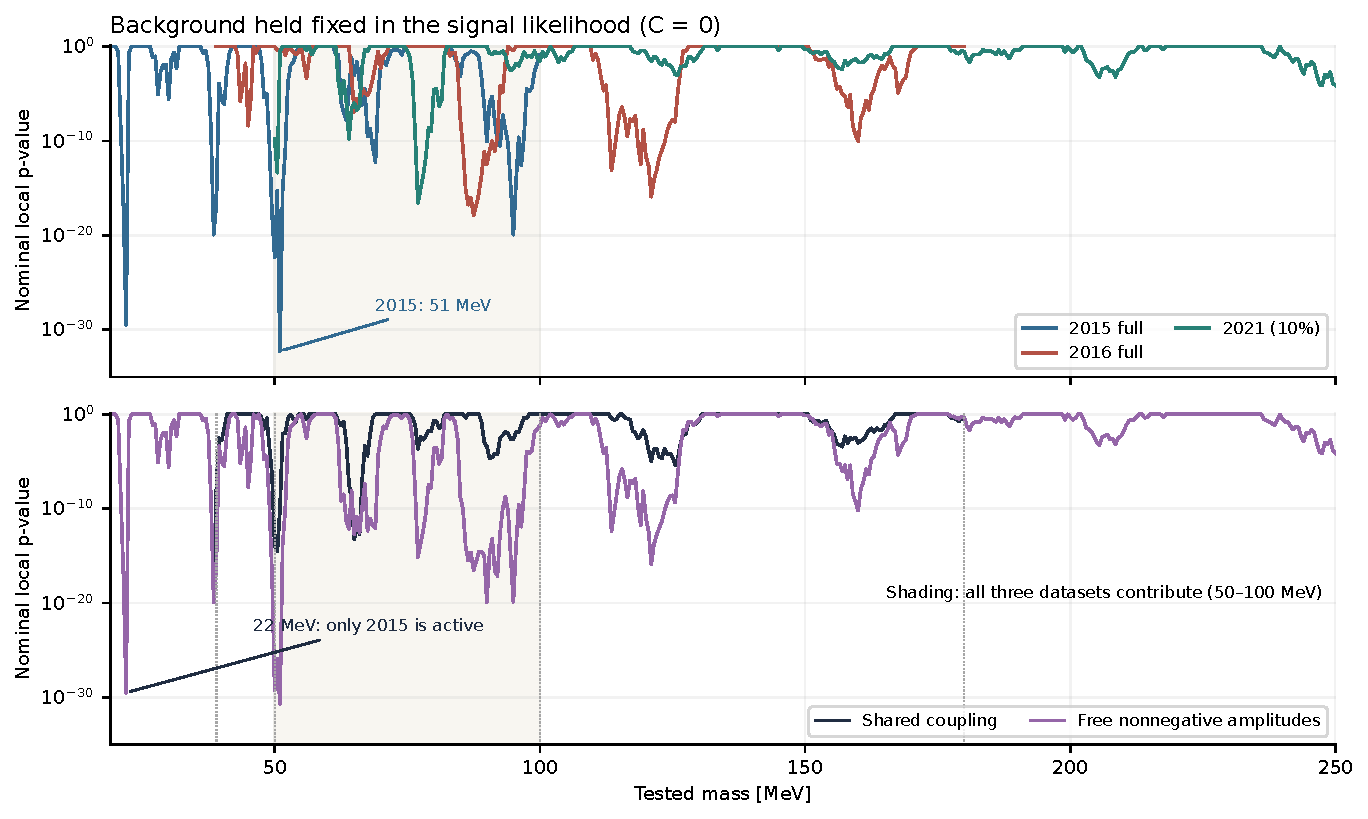
\includegraphics[width=.96\linewidth]{../figures/fixed_background_curves.pdf}
\caption{Computed nominal local probabilities with background covariance set
to zero in the likelihood. The shaded all-three overlap and the changing
union membership are explicit. Very small plotted probabilities are nominal
mappings; direct null calibration is reported in Table~\ref{tab:c0-peaks}.}
\end{figure}

\section*{The new calculation: background fixed inside the signal likelihood}
I have now computed $C=0$ fits for 2015 full, 2016 full and 2021 10\%, and two
combinations. At every mass, the inherited GP recomputes the background mean
$b_{dj}$ from that spectrum's sidebands, excluding $\pm2.25\sigma_m$.
The prediction covariance is then omitted \emph{inside the signal likelihood}:
\begin{equation}
 L_d(A_d;m)=\prod_{j\in W_d(m)}
 \operatorname{Pois}\!\left(n_{dj}\mid b_{dj}+A_d S_{dj}(m)\right).
 \label{eq:fixed-likelihood}
\end{equation}
There are no background nuisance parameters. The GP arithmetic mean and
original signal normalization are retained; $A=\epsilon^2/10^{-8}$.

The shared fit uses one common $A$. The independent-amplitude fit uses one
nonnegative amplitude per active dataset at the same mass. The signed root is
\[
 r=\operatorname{sign}(\widehat A)
 \sqrt{2\{\log L(\widehat A)-\log L(0)\}}.
\]
The nominal local mapping is $p_{\rm nom}=\overline\Phi(r)$ for $r>0$.
For $K$ active independent amplitudes,
\begin{equation}
 q_R=\sum_{d=1}^{K}\max(r_d,0)^2,\qquad
 p_{\rm nom}(q_R)=\sum_{k=1}^{K}
 \frac{\binom Kk}{2^K}\,P(\chi_k^2\ge q_R),\quad q_R>0.
 \label{eq:fixed-free-mixture}
\end{equation}
This nominal chi-bar-square mixture does not identify $\sqrt{q_R}$ with $Z$.
Zero one-sided statistics have inclusive $p=1$. These asymptotic mappings need
checking because $b$ was estimated from the sidebands.

Individual domains are 19--100, 39--180 and 50--250 MeV. Combinations search
the 19--250 MeV union with changing membership, and separately the 50--100 MeV
all-three overlap. Every search uses a 0.5 MeV grid; no domain is chosen for
its smaller probability.

\section*{Checking the nominal probabilities without recentering the scan}
The check repeats the GP prediction and fit on 256 complete Poisson spectra
from the frozen v5.8.2 sources. Each toy has its own sideband estimate, held
fixed only inside its likelihood. Draws are coherent across mass and are
paired with the profiled comparison. This extension uses direct Poisson scans,
not a new significance-field GP approximation.

No offset is subtracted and no response width rescales the root. Global
ordering uses the largest positive raw root for individual/shared fits, and
$\max_m[-\log p_{\rm nom}(q_R(m);K(m))]$ for free amplitudes. The latter accounts
for changing $K$ without reference centering. Observed and toy scans use
identical statistics, grids and domains.

Local tails count exceedances at fixed mass; global tails compare search
maxima. Clopper--Pearson intervals describe sampling uncertainty conditional
on the fixed sources. Zero of 256 exceedances gives only the one-sided 95\%
upper bound $p<0.01163$, not a resolved rare probability.

\section*{The nominated regions under this likelihood}
At 66 MeV the shared root is 7.251, whereas at 92 MeV it is 3.853. The free
mixture at 92 MeV gives nominal $Z=8.521$, driven chiefly by the older samples:
the individual raw roots are 6.371, 6.160 and 0.874. At 78 MeV the roots are
$-8.157$, $-5.200$ and $+7.552$; the free statistic keeps the positive 2021
component and therefore does not establish cross-campaign agreement.

\begin{table}[htbp]\centering\small
\begin{tabular}{rrrrr}\toprule
Mass [MeV] & Shared $p_{\rm nom}$ & Local $k/256$ & Free $p_{\rm nom}$ & Local $k/256$\\\midrule
66 & $2.07\times10^{-13}$ & 0/256 & $2.93\times10^{-13}$ & 3/256\\
78 & $2.06\times10^{-3}$ & 31/256 & $4.85\times10^{-13}$ & 3/256\\
90.5 & $2.24\times10^{-5}$ & 6/256 & $1.73\times10^{-15}$ & 2/256\\
91 & $2.71\times10^{-5}$ & 8/256 & $6.52\times10^{-14}$ & 5/256\\
92 & $5.83\times10^{-5}$ & 7/256 & $7.89\times10^{-18}$ & 1/256\\
\bottomrule\end{tabular}
\caption{Actual combined fits and fixed-mass Poisson checks at the requested
anchors. These counts estimate local conditional tails, not discovery
probabilities after choosing a mass. Zero counts are bounds, as described
above. Every individual and combined row, including global tails at these
thresholds, is saved in the full CSV.}
\label{tab:c0-anchors}
\end{table}

\section*{Why the nominal increase is not a significance gain}
At shared 66 MeV, the toy root has mean $-0.060$ and SD 2.730; its deterministic
root is only 0.060. The nominal 5\% test rejects 59/256 null spectra (23.0\%),
and the nominal 1\% test rejects 43/256 (16.8\%). The same profiled raw-root
toys have SD 1.054. This is missing background-estimation variability
\emph{before} the look-elsewhere effect, even where the mean offset is negligible.
At 22 MeV, both effects matter: the null mean is 3.972 and SD is 3.743.
No correction was applied to the observed roots to produce these comparisons.

\clearpage
\begin{figure}[!ht]\centering
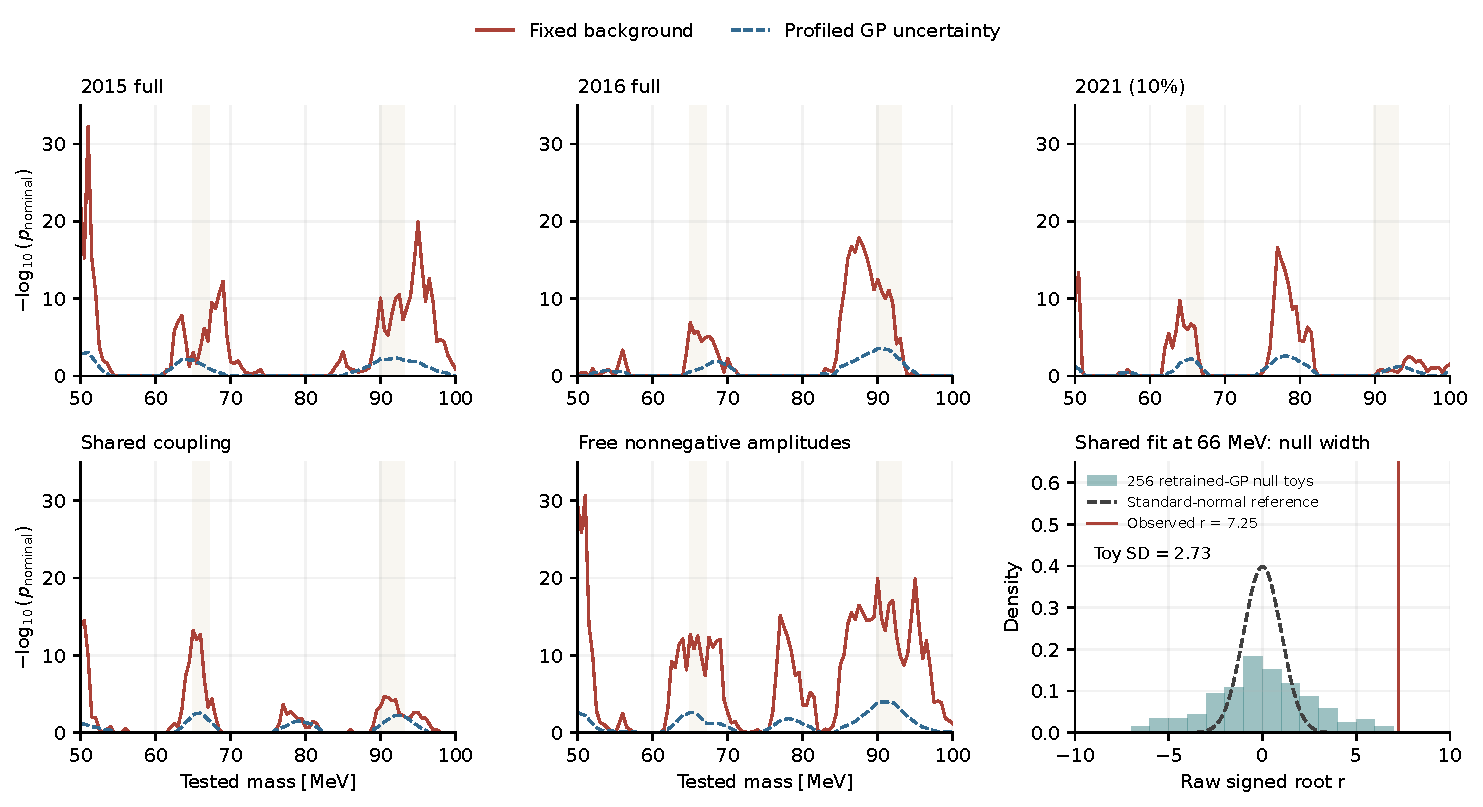
\includegraphics[width=.96\linewidth]{../figures/fixed_background_comparison.pdf}
\caption{The first five panels compare nominal local mappings for the new
$C=0$ fits and the inherited profiled \emph{raw} fits, with no reference
centering in either. The sixth panel compares the direct shared 66 MeV
null-root distribution with a standard normal. Its broad width exposes a
local calibration failure before any search-multiplicity correction.}
\end{figure}

The ratio of a global probability to one of these tiny nominal local
probabilities is therefore not a pure trials factor. Raw ordering remains a
well-defined conditional test, but its varying null width across mass gives
uneven sensitivity. For example, the 92 MeV overlap-global counts are 237/256
shared and 129/256 free, despite its small nominal tails.

My judgement is that the $C=0$ branch is informative about model dependence,
but its nominal improvement is not evidence for a stronger discovery.
Using matched raw tests, the free union gives 48/256 global exceedances here
versus 11/256 when profiled; the shared all-three search gives 38/256 versus
27/256. There is no uniform gain across methods or domains. Any decision to
adopt $C=0$ should compare calibrated power under specified background and
signal ensembles, not select its more striking observed curve. These checks
still condition on a source derived from the observed spectra; source
uncertainty, source learning and prior method choices remain outside their
calibration.
